
\chapter{Lo \textit{stage}}
\label{cap:lo-stage}



\section{Il ruolo degli stage nell'azienda}
Zero12 crede fortemente nella collaborazione tramite \textit{stage} con gli studenti dell'Università di Padova. Grazie all'evento \gls{stageItg}, un evento promosso da Confindustria Veneto Est e l'Università degli studi di Padova, l'azienda permette agli studenti di svolgere progetti di \textit{stage} presso la loro sede.
Gli stage per l'azienda, rappresentano una doppia opportunità. Da una parte, hanno modo di inserire nuove figure professionali nel proprio organico, dall’altra gli studenti hanno la possibilità di inserirsi nel mondo del lavoro e poter applicare le proprie conoscenze acquisite durante il percorso di studi.
Durante le otto settimane di \textit{stage} ho avuto l’occasione di conoscere quasi tutti i membri dell’azienda, comprendere il loro metodo di lavoro e mettere in pratica le mie conoscenze. Il mio percorso è stato guidato dal \textit{tutor} aziendale che mi è stato assegnato, che coordinava le attività da svolgere e che mi forniva supporto in caso di dubbi o problemi. 
L'accoglienza e l'ambiente di lavoro sono molto positivi, dimostrando una grande attenzione nei confronti degli stagisti. 
Questa attenzione è testimoniata anche dalla presenza di molti dipendenti che attualmente lavorano in azienda dopo aver svolto uno \textit{stage} in Zero12.
I progetti assegnati durante gli \textit{stage} vengono concepiti in base a delle reali esigenze interne all’azienda. Essi sono mirati a migliorare la comunicazione tra i collaboratori, automatizzare delle attività manuali e a migliorare la qualità del lavoro svolto.

\section{Introduzione ai progetti}
Durante il mio \textit{stage} ho avuto modo di lavorare non solo al progetto inizialmente proposto, ma anche allo sviluppo di un progetto aggiuntivo, strettamente correlato al primo.
Lo sviluppo di questi due progetti rappresenterebbe un grande vantaggio per l'azienda, ovvero:
\begin{itemize}
    \item \textbf{Prototipi funzionanti}: grazie allo sviluppo di entrambi i progetti, l'azienda avrebbe a disposizione due prototipi funzionanti che dimostrano tutte le potenzialità dei sistemi. Entrambi i progetti utilizzato tecnologie e servizi con cui l'azienda è \textit{partner}.
    \item \textbf{Presentazione ai cliente}: nel caso in cui un cliente si rivolgesse a Zero12 per implementare sistemi simili a quelli che ho sviluppato, l'azienda avrebbe già un prototipo da presentare, che grazie alla sua flessibilità, può essere facilmente adattato alle specifiche del cliente.
    \item \textbf{Utilizzo di IA Generativa}: l'utilizzo della \gls{iaGenerativag}, un ramo dell'intelligenza artificale in grado di generare testo coerente al contesto,  è un punto importante per entrambi i progetti. Questa tecnologia sta diventando sempre più diffusa in diversi ambiti e grazie al suo utilizzo garantisce che questi sistemi siano all'avanguardia.
\end{itemize}
\noindent
Di seguito descrivo il progetto inizialmente proposto dall'azienda all'evento \gls{stageItg} e il progetto aggiuntivo concepito e sviluppato durante lo \textit{stage}.
\subsection{Sistema di proposte di risoluzioni a \textit{ticket} Jira} \label{sec:spiegazioneJira}
L'idea del progetto nasce come strumento che l'azienda può utilizzare per velocizzare il supporto tecnico all'interno dell'azienda, che può essere estesa anche ai suoi clienti. Per comprendere l'idea del progetto, immaginiamo un'azienda che produce e commercializza componenti \textit{hardware}. 
Nel caso di problematiche con la componente acquistata, il cliente chiama il servizio clienti dell'azienda, e l'operatore inserisce un \textit{ticket} all'interno dell'\gls{its} aziendale, che nel contesto del progetto è Jira. Immaginando questa iterazione tra cliente e addetto al servizio clienti per molte volte nel corso degli anni, i \textit{ticket} inseriti all'interno del sistema saranno numerosi e molto simili tra loro. 
Questo implica che in caso di nuovi \textit{ticket} inseriti, è molto probabile che ci siano \textit{ticket} simili già risolti in passato. 
Ed è qui che da Zero12 nasce l'idea di creare un sistema di proposte di risoluzioni automatiche per i \textit{ticket} inseriti all'interno di un \gls{its}, che permetta di velocizzare il processo di risoluzione del problema. Le proposte di risoluzione vengono generate grazie all'utilizzo della \gls{iaGenerativag}, in base al contesto dei \textit{ticket} risolti in precedenza.
Di seguito in figura \ref{fig:ideaJira} mostro uno schema che rappresenta l'idea del progetto principale.

\begin{figure}[H]
    \centering
    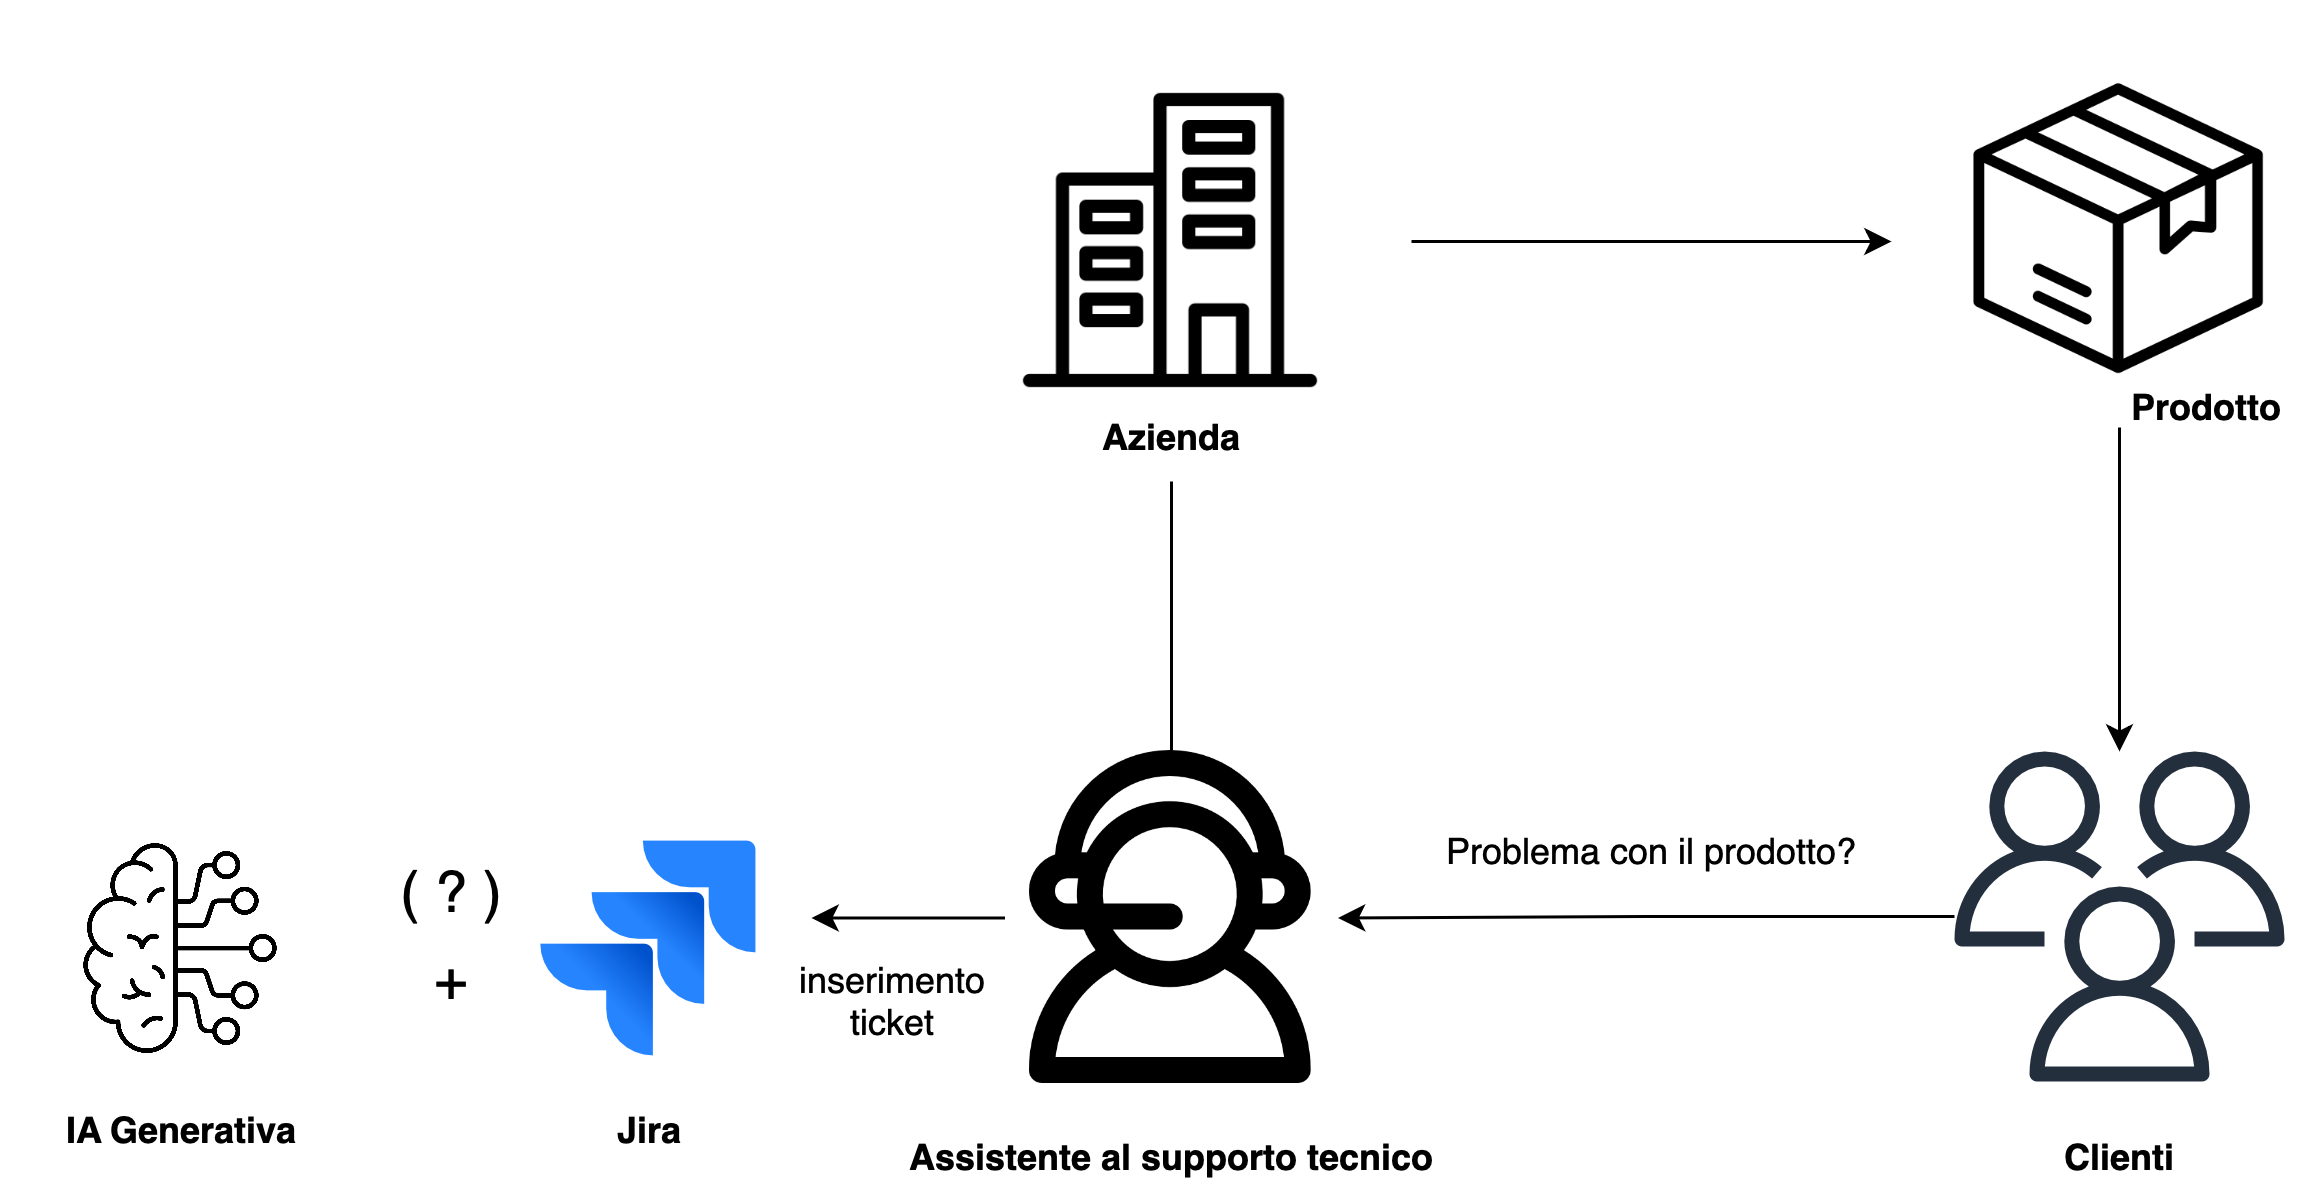
\includegraphics[width=0.95\textwidth]{ideaJira.png}
    \caption{Schema che rappresenta l'idea del progetto principale}
    \small \textbf{Fonte:} \href{https://www.flaticon.com/free-icon/company_4812244}{Icona azienda: https://www.flaticon.com} \href{https://www.flaticon.com/free-icon/box_4601560}{Icona prodotto: https://www.flaticon.com} \href{https://www.flaticon.com/free-icon/assistant_1442194}{Icona assistente: https://www.flaticon.com} \href{https://www.creativefabrica.com/it/product/ai-brain-outline-icon/} {Icona IA Generativa: https://www.creativefabrica.com}

    \label{fig:ideaJira}
\end{figure}
\subsubsection{Benefici del sistema di proposte di risoluzioni}
Il sistema di proposte di risoluzioni a \textit{ticket} Jira, permette di ottenere diversi benefici, qui di seguito elencati:
\begin{itemize}
    \item \textbf{Risposte più veloci}: gli addetti al supporto tecnico possono risolvere le nuove problematiche più velocemente, grazie alle proposte di risoluzione che il sistema genera.
    \item \textbf{Apprendimento continuo}: il sistema permette di apprendere continuamente dai \textit{ticket} risolti in passato, integrando nuove informazioni e conoscenze per generare proposte di risoluzione sempre più precise e dettagliate.
    \item \textbf{Supporto decisionale}: il sistema permette di supportare gli addetti al supporto tecnico nella presa di decisioni, fornendo proposte di risoluzione che possono essere utilizzate come spunto per risolvere il problema.
    \item \textbf{Vantaggi del \textit{cloud}}: il sistema è stato sviluppato utilizzando le tecnologie e i servizi di cui l'azienda è \textit{partner}. Come descritto nella sezione \ref{sec:azienda}, l'azienda è specializzata nello sviluppo di applicazioni \textit{cloud}, e il sistema di proposte di risoluzioni sfrutta proprio queste tecnologie. Questo permette di avere un sistema scalabile e flessibile.
\end{itemize}
\subsection{\textit{Chatbot} per proposte di risoluzioni}
Durante lo sviluppo del progetto descritto nel paragrafo precedente, da parte del mio \textit{tutor} aziendale, è nata l'idea di creare un ulteriore strumento che permetta di svolgere la stessa funzionalità del sistema di proposte di risoluzioni, ma in modo differente. Lo strumento aggiuntivo è un \textit{chatbot} che permette di generare proposte di risoluzione, in base al testo di un \textit{ticket} inserito all'interno della chat. 
Sempre grazie all'utilizzo della \gls{iaGenerativag}, il \textit{chatbot} genera proposte di risoluzione in base al contesto dei \textit{ticket} risolti in precedenza. A differenza del sistema Jira, il \textit{chatbot} propone le risoluzioni in modo più descrittivo e dettagliato, e permette di interagire con l'assistente virtuale, per ottenere informazioni più dettagliate sulle proposte di risoluzione.
\begin{figure}[H]
    \centering
    
\includegraphics[width=0.95\textwidth]{ideaChatbot.png}
    \caption{Schema che rappresenta l'idea del progetto aggiuntivo}
    \label{fig:ideaChatbot}
    \small \textbf{Fonte:} \href{https://uxwing.com/chatbot-icon/}{Icona chatbot: https://uxwing.com} \href{https://www.iconfinder.com/icons/351012/field_input_search_icon}{Icona \textit{input} : https://www.iconfinder.com} \href{https://www.flaticon.com/free-icon/text-file_5116156} {Icona testo: https://www.flaticon.com}
\end{figure}
\subsubsection{Benefici del \textit{chatbot}}
Il \textit{chatbot} per proposte di risoluzioni,  pur non disponendo dei vantaggi del \textit{cloud}, permette di ottenere diversi benefici oltre a quelli che il sistema di proposte precedentemente descritto possiede. Tali benefici sono qui di seguito elencati:
\begin{itemize}
    \item \textbf{Interazione più naturale e intuitiva}: il \textit{chatbot} permette di interagire con l'assistente virtuale attraverso un'interfaccia intuitiva e semplice. L'utente può porre domande specifiche, richiedere chiarimenti sulle proposte e ottenere risposte immediate.
    \item \textbf{Flessibilità e adattabilità}: il \textit{chatbot} potrebbe essere integrato in diversi canali di messagistica, rendendolo uno strumento flessibile e adattabile alle esigenze dell'utente. Nel contesto del progetto, il \textit{chatbot} potrebbe assistere il cliente per risolvere le problematiche più semplici senza la necessità di contattare il servizio clienti.
    \item \textbf{Informazioni più dettagliate}: Il chatbot, grazie alla sua capacità di generare risposte descrittive e dettagliate, può fornire agli operatori informazioni più approfondite rispetto alle semplici proposte di risoluzione generate dal sistema Jira.
\end{itemize}

\section{Obiettivi} \label{sec:obiettiviStage}
\subsection{Obiettivi aziendali}
Durante i primi giorni di \textit{stage} ho definito assieme al mio \textit{tutor} aziendale gli obiettivi del progetto.
Di seguito nella tabella elenco gli obiettivi da raggiungere:
\renewcommand{\arraystretch}{2}
\begin{longtable}{|p{10cm}|p{2cm}|}
    \hline
    \rowcolor{tableheader}\textbf{Obiettivo} & \textbf{Importanza} \\
    \hline
    \endfirsthead

    \rowcolor{tableheader}\textbf{Obiettivo} & \textbf{Importanza} \\
    \hline
    \endhead

    \hline
    \endfoot

    \hline
    \endlastfoot
    \rowcolor{tableoddrow} Studio delle tecnologie e studio di fattibilità & Obbligatorio \\
    \hline
    \rowcolor{tableevenrow} Creazione dati di \textit{mock} da inserire nell' \gls{its} Jira & Obbligatorio \\
    \hline
    \rowcolor{tableoddrow} Reperimento dei ticket su Jira e salvataggio su \textit{database} mongoDB & Obbligatorio \\
    \hline
    \rowcolor{tableevenrow} Aggiornamento costante del \textit{database} a nuovi \textit{ticket} risolti su Jira & Obbligatorio \\
    \hline
    \rowcolor{tableoddrow} Eseguire \gls{rag}, una tecnica avanzata di elaborazione di linguaggio naturale, sui \textit{ticket} salvati & Obbligatorio \\
    \hline
    \rowcolor{tableevenrow} \textit{Benchmark} su vari modelli per la generazione della risposta & Obbligatorio \\
    \hline
    \rowcolor{tableoddrow} Creazione del sistema di proposte di risoluzione su Jira & Obbligatorio \\
    \hline
    \caption{Obiettivi da raggiungere per il sistema di proposte di risoluzione su Jira}
    \label{tab:obiettiviJira}
\end{longtable}
\noindent
Durante lo sviluppo del progetto, grazie il buon andamento che ho avuto, al mio \textit{tutor} aziendale è nata l'idea di sviluppare il progetto aggiuntivo relativo al \textit{chatbot} per le proposte di risoluzione.
Di seguito elenco gli obiettivi extra da raggiungere:
\begin{longtable}{|p{10cm}|p{2cm}|}
    \hline
    \rowcolor{tableheader}\textbf{Obiettivo} & \textbf{Importanza} \\
    \hline
    \endfirsthead

    \rowcolor{tableheader}\textbf{Obiettivo} & \textbf{Importanza} \\
    \hline
    \endhead

    \hline
    \endfoot

    \hline
    \endlastfoot
    \rowcolor{tableoddrow} Studio delle tecnologie e studio di fattibilità & Desiderabile \\
    \hline
    \rowcolor{tableevenrow} Implementazione interfaccia \textit{web} per l'interrogazione del \textit{chatbot} & Desiderabile \\
    \hline
    \rowcolor{tableoddrow} Impostazione di un formato di domanda dell'utente da seguire & Desiderabile \\
    \hline
    \caption{Obiettivi da raggiungere del progetto \textit{chatbot}}
    \label{tab:obiettiviChatbot}
\end{longtable}

\subsection{Obiettivi personali} \label{sec:obiettiviPersonali}
Prima dell'inizio dello \textit{stage}, mi sono prefissato degli obiettivi che riguardassero gli aspettivi che volevo curare durante il tirocinio. Di qui seguito elenco gli aspetti che ho tenuto in considerazione:
\begin{itemize}
    \item \textbf{Conoscenza delle metodologie aziendali}: acquisire nuove conoscenza e competenze riguardanti le metodologie di sviluppo \textit{software} e dei processi aziendali. 
    \item \textbf{Conoscenze tecniche}: sviluppare competenze in merito alle tecnologie utilizzate, permettondomi di mettere in pratica le conoscenze acquisite durante il mio percorso di studi
    \item \textbf{\textit{Problem solving}}: migliorare il mio approccio alla risoluzione dei problemi, migliorando la mia capacità di analisi e di risoluzione rispettando i vincoli imposti.
    \item \textbf{Introduzione al mondo del lavoro}: Comprendere le dinamiche e l'organizzazione lavorativa di un'azienda operante in questo settore.
\end{itemize}
Questa è stata la mia prima vera esperienza lavorativa in un'azienda del settore informatico, e ho voluto sfruttare al massimo questa opportunità per crescere professionalmente e personalmente.
Nella seguente tabella, riporto gli obiettivi personali secondo la seguente notazione:
\begin{center}
    \textbf{OP-I}
\end{center}
dove:
\begin{itemize}
    \item \textbf{OP}: abbreviazione di Obiettivo Personale
    \item \textbf{I}: numero intero positivo incrementale, identificativo dell'obiettivo
\end{itemize}

\renewcommand{\arraystretch}{2}
\begin{longtable}{|p{2cm}|p{9cm}|}
    \hline
    \rowcolor{tableheader}\textbf{Codice Obiettivo} & \textbf{Descrizione dell'Obiettivo Personale} \\
    \hline
    \endfirsthead

    \rowcolor{tableheader}\textbf{Codice Obiettivo} & \textbf{Descrizione dell'Obiettivo Personale} \\
    \hline
    \endhead

    \hline
    \endfoot

    \hline
    \endlastfoot
    \rowcolor{tableoddrow} OP-1 & Sviluppare competenze con strumenti di comunicazione e collaborazione aziendali come Slack e GitHub \\
    \hline
    \rowcolor{tableevenrow} OP-2 & Sviluppare competenze con i \textit{framework} utilizzati, come Serverless \textit{framework} e Streamlit \\
    \hline
    \rowcolor{tableoddrow} OP-3 & Sviluppare competenze con nuovi linguaggi di programmazione come TypeScript e Python. \\
    \hline
    \rowcolor{tableevenrow} OP-4 & Sviluppare competenze con le tecnologie offerte da \gls{aws}. \\
    \hline
    \rowcolor{tableoddrow} OP-5 & Partecipare ai processi di sviluppo \textit{software} in ambito aziendale. \\
    \hline
    \rowcolor{tableevenrow} OP-6 & Comprendere i ritmi e le dinamiche di un lavoro in questo settore. \\
    \hline
    \caption{Obiettivi personali durante lo \textit{stage}}
    \label{tab:obiettiviPersonali}
\end{longtable}
\section{Vincoli dello \textit{stage}}
\subsection{Vincoli tecnologici}
I vincoli tecnologici imposti dall'azienda includevano l'utilizzo delle tecnologie utilizzate nello \textit{stack} aziendale, descritte nella sezione \ref{sec:tecnologie}. 
In aggiunta, mi è stato chiesto di utilzzare le \gls{api} che fornisce Jira, per il caricamento di \textit{ticket} di \textit{mock} all'interno di un progetto Jira, e per il recupero dei \textit{ticket} risolti da inserire nel \textit{database}.
Mi è stato inoltre chiesto di utilizzare i \textit{webhook} di Jira, per impostare un \textit{trigger} che invii eventi al sistema che ho sviluppato, in modo che alla chiusura di un \textit{ticket} su Jira, il sistema aggiorna automaticamente il \textit{database} con il nuovo \textit{ticket} completato.
\subsection{Vincoli di rendicontazione}
Durante il mio periodo di \textit{stage}, l'azienda mi ha richiesto la stesura di una tabella riassuntiva dei risultati del \textit{benchmark} dei vari modelli testati. I risultati dei vari modelli sono stati assegnati secondo metriche di valutazione da me impostate e motivate, descritti nella sezione \ref{sec:rag}.
Mi è stato richiesta la stesura di un documento in cui spiego le scelte adottate durante lo sviluppo del progetto, indicando le componenti sviluppate, le librerie utilizzate e le motivazioni dietro le scelte fatte.
Mi è stata richiesta anche la stesura di un manuale utente, in cui spiego come configurare correttamente il sistema su Jira, e come utilizzarlo. Quest'ultimo documento comprende anche una sezione in cui descrivo il corretto utilizzo del \textit{chatbot}.\\
Durante l'ultima settimana infine, mi è stato richiesto di preparare una presentazione sui progetti sviluppati, che avrei dovuto esporre a tutti i membri presenti dell'azienda. Questa presentazione doveva contenere le idee dei progetti, la loro importanza, i risultati ottenuti e le possibile evoluzioni future.
\subsection{Vincoli temporali}
Il progetto di \textit{stage} è stato ideato per essere sviluppato in otto settimane, limite massimo di tempo per lo svolgimento del tirocinio curricolare. Nello specifico, è stato programmato in giornate lavorative da 8 ore ciascuna, per un totale di non più di 320 ore, suddivise in 40 ore settimanali.

\subsection{Vincoli organizzativi}
L'organizzazione dello \textit{stage} è stata fondamentale per garantire un percorso valido e proficuo. Questa organizzazione provvedeva un costante allineamente tra gli attori che di seguito elenco:
\begin{itemize}
    \item \textbf{\textit{Tutor} aziendale}: durante tutto il periodo di \textit{stage}, il contatto con il \textit{tutor} aziendale doveva essere costante, al fine di garantire un monitoraggio costante dell'avanzamento del progetto che gli obiettivi prefissati venissero raggiunti. 
    \item \textbf{Comunicazioni con il relatore}: il contatto con il relatore universitario doveva essere costante, in modo da allineare l'andamento dello \textit{stage} e il suo stato di avanzamento. A tale scopo, ogni 5 giorni lavorativi, inviavo un resoconto delle attività svolte, degli obiettivi raggiunti e delle pianificazioni per il periodo successivo.
\end{itemize}
\section{Scelta dello \textit{stage}} \label{sec:sceltaStage}
Durante l'evento \gls{stageItg} ho avuto modo di connoscere numerose azienda, e di ascoltare i loro progetti di \textit{stage}. 
La scelta del progetto di Zero12 è stata basata su una serie di fattori che descrivo qui di seguito:
\begin{itemize}
    \item \textbf{Tema del progetto}: il progetto sul supporto tecnico facilitato con l'aiuto della \gls{iaGenerativag}, come descritto nel paragrafo \ref{sec:spiegazioneJira}, mi ha subito colpito, in quanto mi avrebbe permesso di approfondire l'utilizzo di questa tecnologia, sempre più diffusa in vari settori. Ho scelto questo progetto anche per la sua utilità in ambito aziendale e la possibilità di poterlo estendere a clienti reali.
    \item \textbf{Prima impressione}: come ho descritto all'inizio del paragrafo, ho avuto modo l'opportunità di parlare con diverse aziende. Il colloquio che ho avuto con Zero12 è stato quello che mi è rimasto più impresso, in quanto si sono dimostrati molto disponibili nel rispondere alle mie domande, molto chiari nelle loro descrizioni e molto accoglienti. Dopo il colloquio, e a seguito dell'ottima impressione che ho ricevuto, mi sono interessato maggiormente al progetto da loro proposto.
    \item \textbf{Tecnologie utilizzate}: i giorni prima l'evento, ho avuto modo di esaminare le tecnologie richieste per lo sviluppo del progetto. Tra queste, vi erano tecnologie a me già familiari, come Typescript, Node.js e MongoDB. Il restante delle tecnologie, erano legate ai servizi \textit{cloud} offerte da \gls{aws}, che ho avuto modo di accennare durante il mio percorso scolastico. Ho scelto questo progetto anche per la possibilità di approfondire queste tecnologie e di poterle utilizzare in ambito aziendale.
    \item \textbf{\textit{Cloud} e \gls{iaGenerativag}}: come descritto nella sezione \ref{sec:azienda}, Zero12 è specializzata nello sviluppo di applicazioni \textit{cloud} ed è \textit{partner} \gls{aws}. Il progetto inizialmente proposto, utilizzano tecnologie e servizi \gls{aws}, e \gls{iaGenerativag}. Questo aspetto mi ha colpito molto, in quanto mi avrebbe permesso di mettere mano a questo tipo di tecnologie e di poterle utilizzare in un contesto lavorativo.
\end{itemize}
Nelle motivazioni riguardanti la scelta dello \textit{stage}, non ho tenuto in considerazione la posizione geografica delle aziende. L'obiettivo principale era quello di selezionare un progetto con un aspetto formativo e professionale, che mi permettesse di approfondire le mie conoscenze e di metterle in pratica in un contesto lavorativo. Nel caso specifico di Zero12, la sede aziendale distra a circa 40 minuti di auto da dove risiedo.
